با استفاده از محاسبه‌ی هسین مساله را حل می‌کنیم. همچنین برای سادگی به‌جای نمادگزاری مساله، از
$x^\alpha y^\beta$
استفاده می‌کنیم.
\[
\nabla f = \begin{bmatrix}
	\alpha x^{\alpha - 1}y^{\beta}\\
	\beta x^{\alpha}y^{\beta - 1}\\
\end{bmatrix}
\implies
H = x^{\alpha - 2}y^{\beta - 2}\begin{bmatrix}
\alpha (\alpha - 1)y^2 & \alpha \beta xy\\
 \alpha \beta xy & \beta (\beta - 1)x^2\\
\end{bmatrix}
\]
حال دقت کنید که ضریب پشت ماتریس همواره مثبت است. پس برای بررسی $H$ باید دترمینان آن و نیز ضرایب روی قطر را بررسی کنیم. \\
\begin{enumerate}
	\item 
	$H$ مثبت‌نیمه‌معین است اگر و تنها اگر
	\[
	\alpha (\alpha - 1) \ge 0 \land \beta (\beta - 1) \ge 0 \land x^2y^2\alpha \beta (1 - \alpha - \beta) \ge 0
	\]
	در نتیجه اگر 
	$\alpha, \beta > 0$
	باشند که ممکن نیست چون که 
	باید هر دو حداقل ۱ باشند و در نتیجه نامساوی سوم درست نخواهد بود.\\
	اگر هر دو منفی باشند (منظور نامثبت)، مشکلی نداریم چون که نامساوی‌های برقرارند. پس اگر هر دو نامثبت باشند تابع محدب است.
	اگر یکی مثبت و دیگری نامثبت باشد، مثلا $\alpha$ مثبت باشد، در این صورت
	\[
	\alpha (\alpha - 1) \ge 0 \implies \alpha \ge 1, \quad \beta(1 - \alpha - \beta) \ge 0 \implies
	\beta \ge 1 - \alpha 
	\]
	از طرفی دقت کنید که اگر 
	$\alpha \ge 1, \beta \ge 1- \alpha$،
	هر ۳ نامساوی برقرارند. پس یک حالت هم این است که 
	$\alpha\beta \le 0, \alpha + \beta \ge 1$.
	شکل مورد نظر در 
	\ref{fig2:convex}
	آمده است.
	\item 
برای دو شرط اول باید داشته باشیم
\[
\alpha(\alpha - 1) \le 0\land  \beta(\beta - 1) \le 0  \implies1 \ge  \alpha, \beta \ge 0
\]
همچنین  برای شرط سوم باید داشته باشیم
\[
1 - \alpha - \beta \ge 0 \implies \alpha + \beta \le 1
\]
پس مقعر بودن معادل است با
\[
\alpha, \beta \ge 0 \land \alpha + \beta \le 1
\]
شکل مورد نظر در 
\ref{fig2:concave}
آمده است.
\begin{figure}[H]
	\centering
	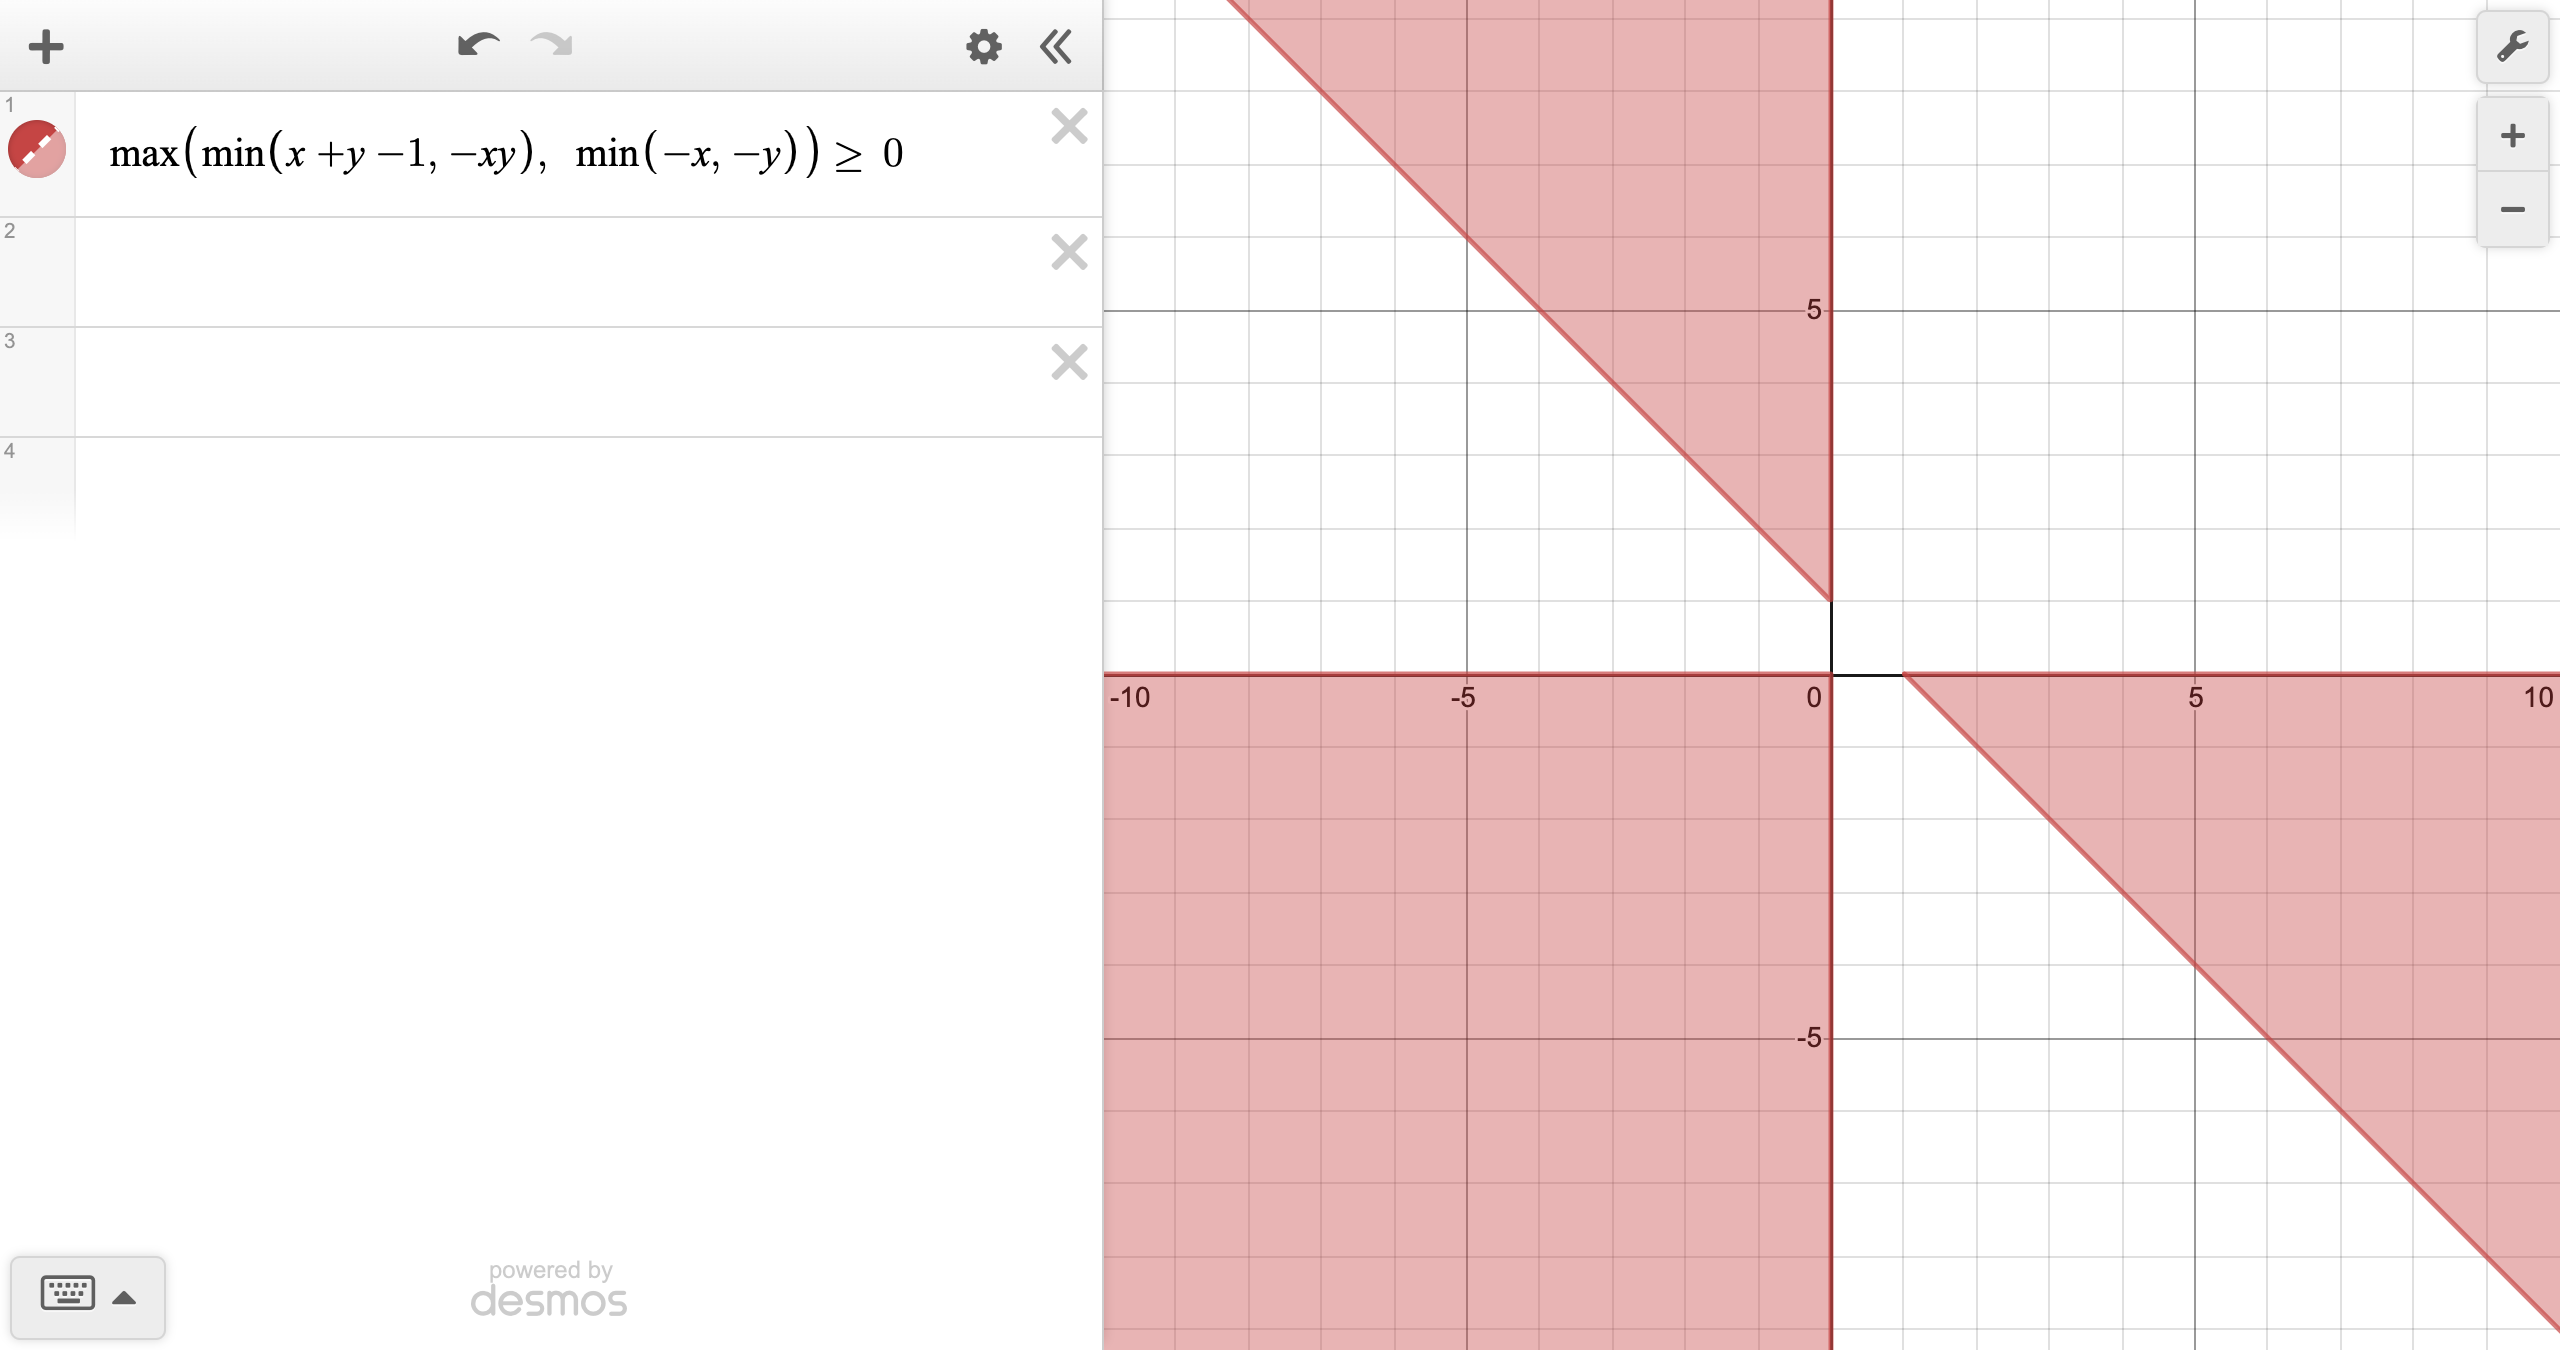
\includegraphics[width=0.9\textwidth]{convex}
	\caption{شکل سوال ۲ الف}
	\label{fig2:convex}
\end{figure}
\begin{figure}[H]
	\centering
	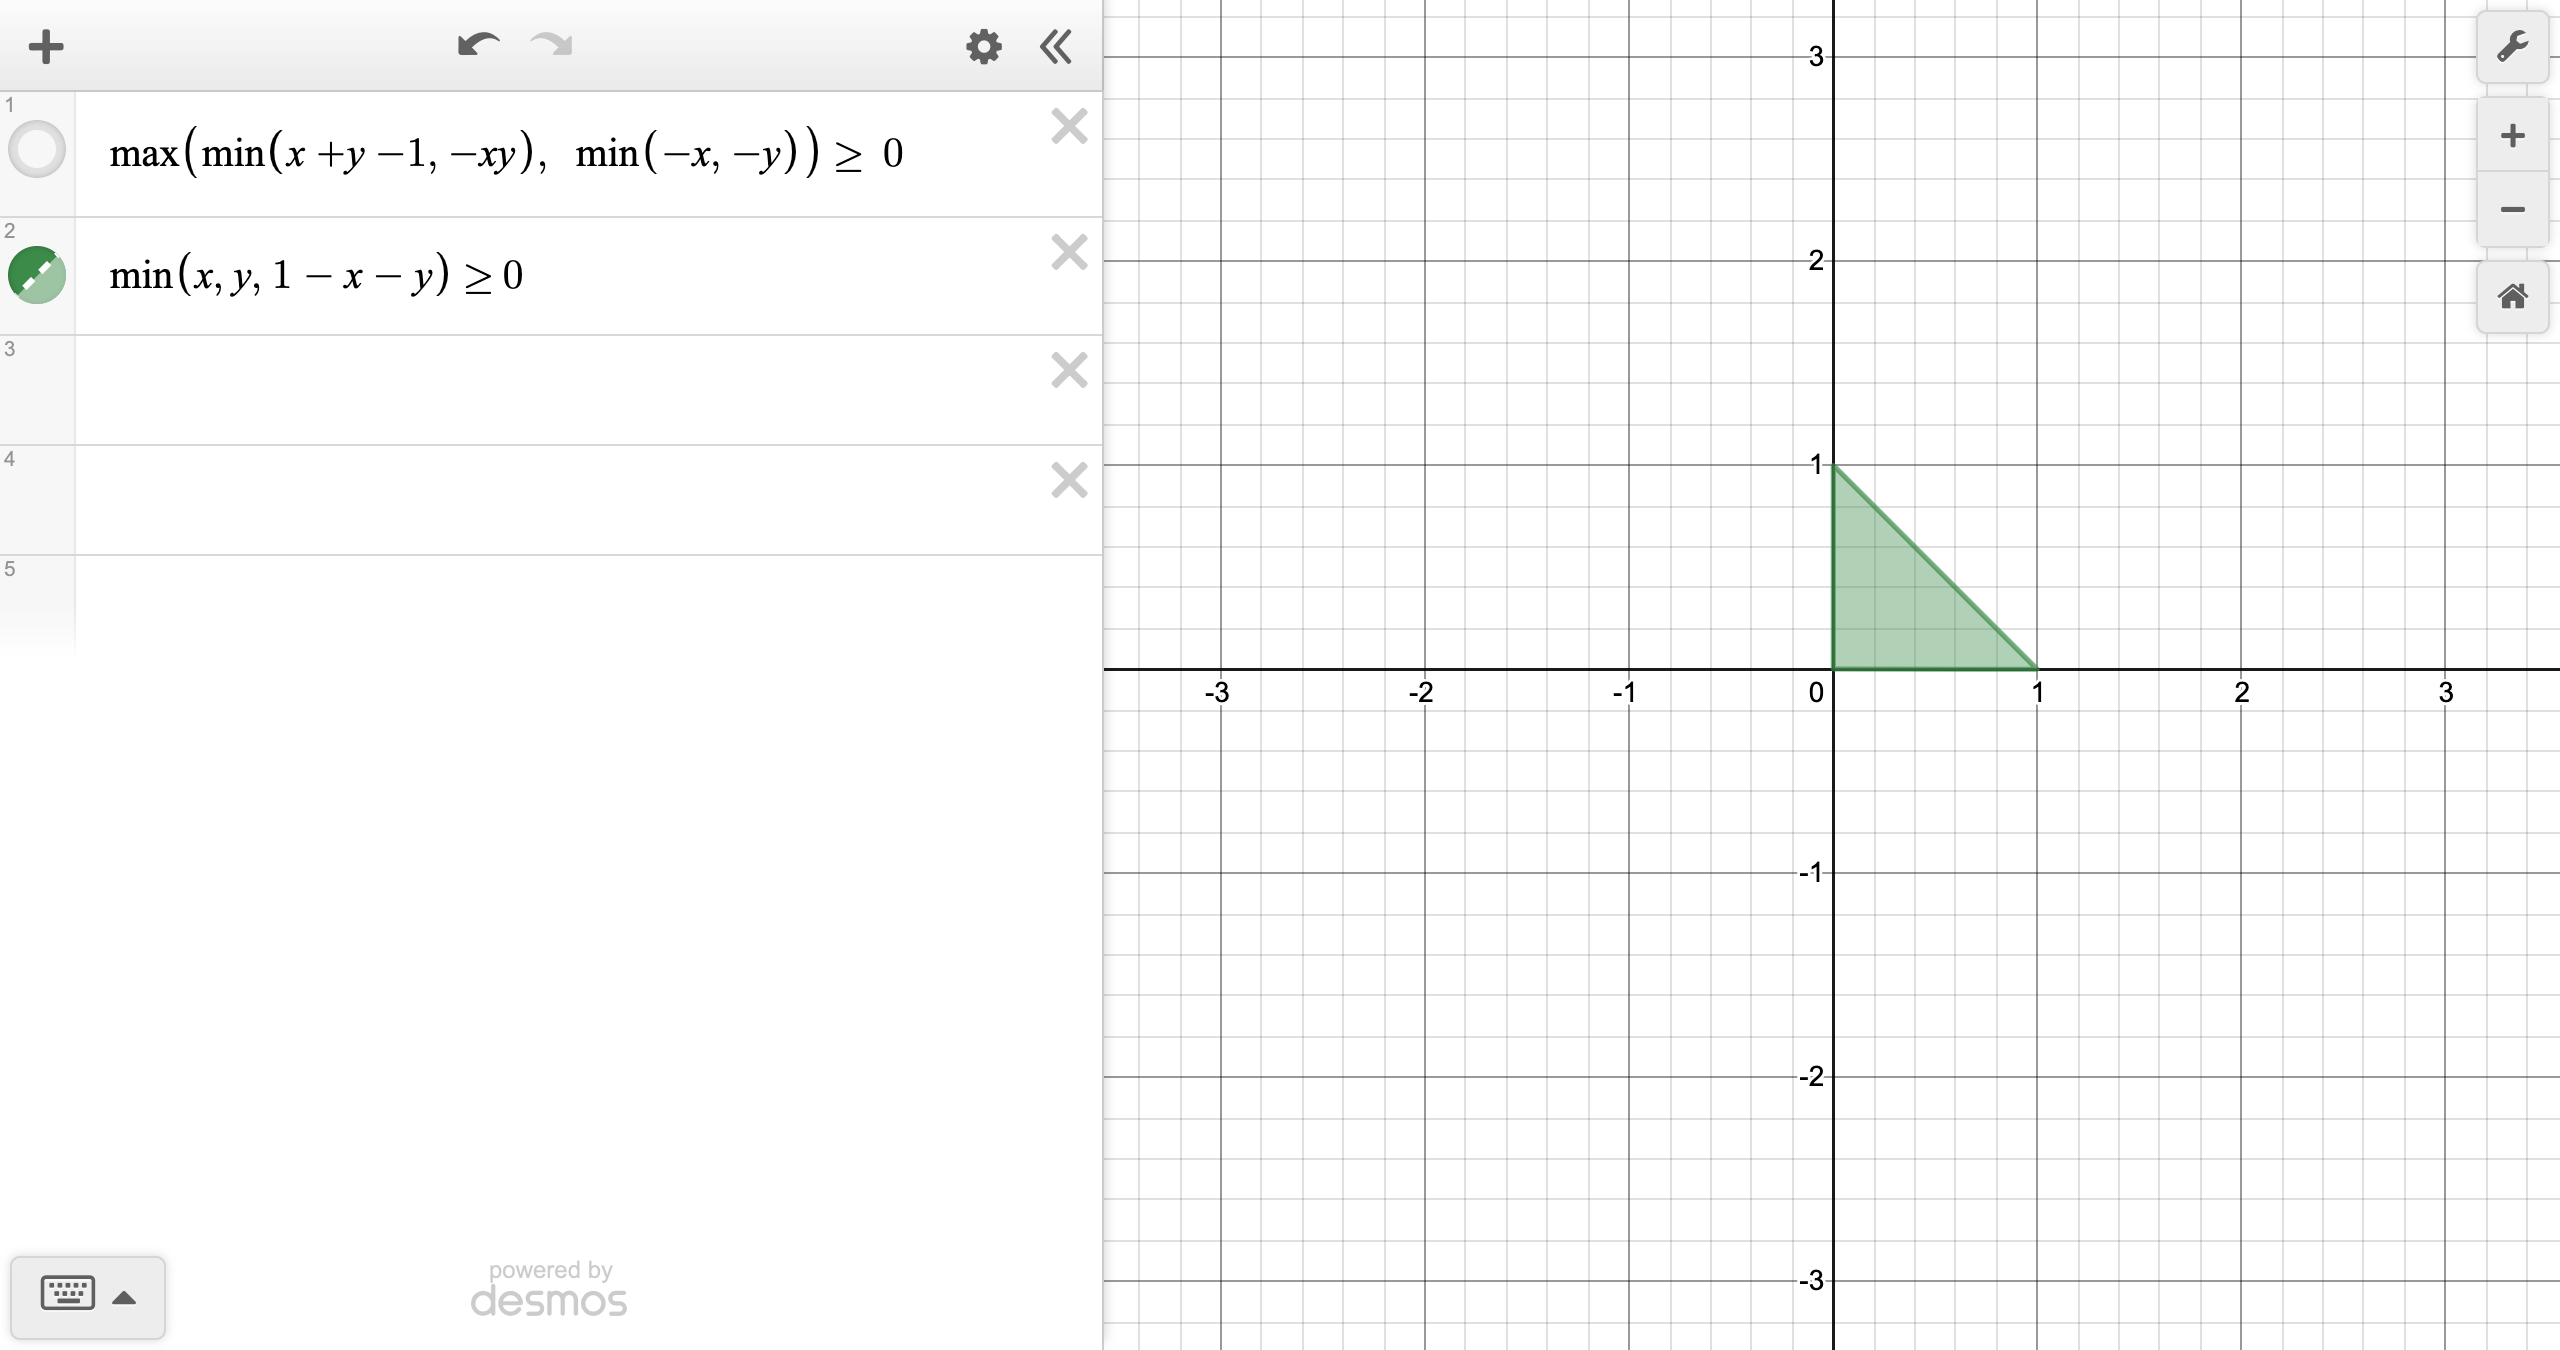
\includegraphics[width=0.9\textwidth]{concave}
	\caption{شکل سوال ۲ ب}
	\label{fig2:concave}
\end{figure}
\end{enumerate}
حال به حل بخش امتیازی می‌پردازیم. به این منظور، دقت کنید که هسین روی قطر برابر است با
\[
(\prod x_i^{\alpha_i} )\frac{\alpha_i (\alpha_i - 1)}{x_i^2}
\]
و خارج از قطر برابر است با
\[
(\prod x_i^{\alpha_i} )\frac{\alpha_i \alpha_j}{x_ix_j}
\]
که چون 
$(\prod x_i^{\alpha_i} )$
مثبت است، می‌توان آن را در نظر نگرفت. با این توصیفات، به حل مساله می‌پردازیم. 
\textbf{ابتدا مقعر بودن و سپس محدب بودن را بررسی می‌کنیم}
\begin{enumerate}
	\item 
اولا دقت کنید که اگر 
$\alpha_i < 0$،
درایه‌ی $i$‌ام روی قطر مثبت خواهد بود. در نتیجه قطعا مقعر نیست. پس
$\alpha \ge 0$.
حال برای هر $v$ دلخواه باید داشته باشیم.

\begin{equation}
\forall v \in R^n : \sum v_i^2\frac{\alpha_i^2 - \alpha_i}{x_i^2} + 2\sum_{i \ne j} v_iv_j\frac{\alpha_i\alpha_j}{x_ix_j} \le 0 \iff 
(\sum v_i\frac{\alpha_i}{x_i})^2 \le \sum \alpha_i\frac{v_i^2}{x_i^2}
\label{eq2:1}
\end{equation}

اگر که داشته باشیم
$\sum \alpha_i \le 1$،
\[
RHS \ge RHS \times \sum \alpha_i = (\sum \alpha_i)(\sum \alpha_i\frac{v_i^2}{x_i^2})
\]
که طبق کوشی شوارتز از
$LHS$
بیشتر است و در نتیجه تابع مقعر است. از طرفی اگر 
\ref{eq2:1}
برای $v$ دلخواه برقرار باشد، داریم
\[
v_i = x_i \implies (\sum \alpha_i)^2 \le (\sum \alpha_i) \implies \sum \alpha_i \le 1
\]
پس تابع مقعر است اگر و تنها اگر
\[
\alpha \ge 0 \land \sum \alpha_i \le 1
\]
\item 
فرض کنید که دو تا از
$\alpha_i$‌ها
مثبت باشند. در این صورت با در نظر گرفتن تصویر روی همان دو متغیر، باید هنوز تابع محدب بماند. اما با توجه به این که در بخش غیرامتیازی ثابت کردیم که اگر محدب باشد همچین چیزی ممکن نیست، این حالت منتفی است. پس یا همه نامثبت‌اند و یا دقیقا یکی مثبت است. اگر همه نامثبت باشند، باید برای هر $v$ دلخواه داشته باشیم (بسط دادن هسین مشابه قبل است)

\begin{equation}
\forall v \in R^n : \sum v_i^2\frac{\alpha_i^2 - \alpha_i}{x_i^2} + 2\sum_{i \ne j} v_iv_j\frac{\alpha_i\alpha_j}{x_ix_j} \ge 0 \iff 
(\sum v_i\frac{\alpha_i}{x_i})^2 \ge \sum \alpha_i\frac{v_i^2}{x_i^2}
\label{eq2:2}
\end{equation}

که همواره برقرار است زیرا سمت راست نامثبت است و سمت چپ نامنفی.
اگر هم دقیقا یکی از 
$\alpha_i$‌ها
مثبت باشد و بقیه نامثبت، با قرار دادن 
$v_i=x_i$
نتیجه می‌گیریم که 
\[
(\sum \alpha_i)^2 \ge \sum \alpha_i
\]
و در نتیجه یا 
$\sum \alpha_i \le 0$،
یا 
$\sum \alpha_i \ge 1$.
در حالت اول، اگر همه‌ی
$x_i$
‌هایی که ضریبشان منفی است را یکی کنیم (یعنی یک متغیر کنیم. این کار ممکن است چون \lr{precomposition} با آفین)،
تابع باید محدب بماند. اما خب محدب نمی‌ماند زیرا الان یک 
$\alpha_i$
مثبت داریم، یک 
$\alpha_i$
نامثبت و جمعشان هم نامثبت است که در شرایط بخش غیرامتیازی صدق نمی‌کند چون در حالت یکی مثبت، یکی نامثبت، باید جمع حداقل ۱ می‌شد.\\
پس در حالت دوم هستیم و در نتیجه 
\[
\sum \alpha_i \ge 1
\]
ثابت می‌کنیم که همین شرایط کافیست. به این منظور ابتدا حالتی که 
$\sum \alpha_i = 1$
است را بررسی می‌کنیم. در این حالت، اگر فرض کنیم که 
$\alpha_n > 0$
و بقیه‌ نامثبت‌اند، می‌دانیم
$x \in R^{n - 1} \to \prod x_i^{\alpha_i}$
محدب است. در نتیجه طبق قانون پرسپکتیو، تابع زیر محدب است
\[
x \in R^{n - 1}, g(t, x) = t\prod((\frac{x_i}{t})^{\alpha_i}) = t^{1 - \sum \alpha_i} \prod x_i^{\alpha_i}
\]
که همان تابع ماست با این تفاوت که به‌جای
$x_n$
از $t$ استفاده کرده‌ایم. پس این حالت حل شد. در حالتی که 
$\sum \alpha_i > 1$
هم می‌توانیم تعریف کنیم
$g(x) = \prod x_i^{\frac{\alpha_i}{\sum \alpha_i}}$.
طبق چیزی که الان ثابت کردیم، 
$g$ محدب است.
پس چون تابع زیر محدب است (چون $\sum \alpha_i \ge 1$) و همچنین صعودی است
\[
x \in R^+, h(x) = x^{\sum \alpha_i}
\]
نتیجه می‌گیریم که تابع اصلی هم محدب است. پس برای این بخش هم ۲ حالت وجود دارد.
حالت اول این که 
\[
\alpha \le 0
\]
و حالت دوم هم این که دقیقا یکی از $\alpha_i$‌ها مثبت است و همچنین
\[
\sum \alpha_i \ge 1
\]
\end{enumerate}